\subsubsection{Pikunda-Munda-Gruppe}\label{sec:PKM-Gr}

Der Pikunda-Munda-Stil beschreibt die älteste in größerem Umfang nachweisbare Keramik im südlichen Teil des Arbeitsgebiets.\footnote{Der älteren Imbonga-Gruppe zurechenbare Stücke fanden sich lediglich in sehr begrenztem Rahmen an zwei Fundstellen am unteren \mbox{Sangha} (Kap.~\ref{sec:IMB-Gr}; Kat.-Nr.~12--13).} Die Beschreibung der morphologischen wie ornamentalen Charakteristika basiert zu großen Teilen auf Inventaren einer in Pikunda am \mbox{Sangha} im Grabungsschnitt PIK~87/1 (Kat.-Nr.~8; Bereich B1/B2) angeschnittenen Grube sowie den drei Befunden MUN~87/2-1-1 (Kat.-Nr.~16), MUN~87/2-1--3 (Kat.-Nr.~17) und MUN~87/3 (Kat.-Nr.~18) in Munda am Likwala-aux-Herbes. Die im Zuge dieser Grabungen erfasste Keramik wurde bereits von \textcites{Eggert.1992}{Eggert.1993} unter der Bezeichnung \enquote{Pikunda-Munda-Horizont} systematisiert. Insgesamt lassen sich 529~GE und 18 ausgezählte Scherben der Pikunda-Munda-Gruppe zuweisen. Knapp zwei Drittel der GE stammen aus den genannten Grabungen, während der Rest (35\,\%) bei Absammlungen rezenter Dorfflächen gefunden wurde.\footnote{Die Fragmentierung von Grabungs- sowie Surveyfunden ist ungefähr gleich. Während der Anteil stark zerscherbter Stücke bei den Surveyfunden geringer ist (4\,\%) als bei den Grabungsfunden (30\,\%), gleicht der höhere Anteil mittelgroßer Fragmente innerhalb der Surveyfunde (73\,\%) gegenüber den Grabungsfunden (50\,\%) das Verhältnis wieder aus. In beiden Kategorien sind fast 80\,\% aller Scherben kleiner als 70\,$\times$\,70\,mm. Komplette Gefäße machen 2\,\% aller in Grabungen gefunden GE aus, während sie nur zu 0,5\,\% bei den Surveyfunden zu beobachten waren. Aus diesen Verhältnissen ergibt sich aber keine grundsätzliche Abweichung hinsichtlich der Fragmentierung der Stücke und der damit verbundenen Frage der Erhaltung zwischen dem keramischen Material aus Grabungen und jenem aus Surveys. In den Surveyinventaren konnten etwa 60\,\% der Stücke sicher der Stilgruppe zugewiesen werden, während innerhalb der Grabungsfunde bis zu 80\,\% der GE sicher angesprochen werden konnten.} Da die Keramik der Pikunda-Munda-Gruppe, wie im Weiteren ausgeführt wird, starke Ähnlichkeiten zur Technologie und den Verzierungstechniken anderer, in ihrem Verbreitungsgebiet vorkommenden Stile wie Ngombe (Kap.~\ref{sec:NGO-Gr}) oder Epena (Kap.~\ref{sec:EPE-Gr}) aufweist, war eine sichere Zuweisung bei Surveyfunden nicht immer möglich. \footnote{Gemeint sind hiermit stark zerscherbte Stücke, die das \textit{Fabric} 1 zeigen und die lediglich Reste einer aus Rillen (Tab.~\ref{tab:Verzierungselemente}: 01) und Riefen (Tab.~\ref{tab:Verzierungselemente}: 02) bestehenden Verzierung aufweisen. \textit{Fabric} 1 ist für sehr viele keramische Stilgruppen des \mbox{Sangha}- und Likwala-aux-Herbes-Gebietes charakteristisch (Tab.~\ref{tab:Fabrics_StilGr_Pct}, Abb.~\ref{fig:Fabrics_Verbreitung}). Die entsprechenden Stücke ließen sich, wenn sie bei Oberflächensurveys gefunden wurden, nur sehr schwer in einem hinreichenden Maße sicher einer Stilgruppe zuweisen.} Das Inventar der Pikunda-Munda-Gruppe umfasst neben 37 komplett oder hinreichend erhaltenen Gefäßen (7\,\%)\footnote{29 der 37 Gefäße stammen aus den in Munda am \mbox{Likwala}-\mbox{aux}-\mbox{Herbes} (Fpl.~304) ausgegrabenen Befunden. Allein zehn Gefäße stammen aus dem Befund MUN~87/2-1-1 (Kat.-Nr.~16; Taf.~91) und 15 Gefäße aus MUN~87/2-1-3 (Kat.Nr.~17; Taf.~92--93). Die Grabung des Befundes PIK~87/1 in Pikunda am \mbox{Sangha} (Fpl.~255) erbrachte nur zwei nahezu vollständige Gefäße (Taf.~44.3, 45.2).} vornehmlich Fragmente von Gefäßwandungen (57\,\%). Randfragmente nehmen nur etwa ein Drittel der Stücke ein (32\,\%), während dezidierte Bodenscherben nur selten beobachtet wurden (4\,\%).

\paragraph{Technologische Merkmale}\hspace{-.5em}|\hspace{.5em}%
Die Keramik der Pikunda-Munda-Gruppe ist von einem Scherben bestimmt, der praktisch keine nichtplastischen Partikel enthält. Bei sichtbaren Partikeln handelte es sich fast ausnahmslos um äußerst feinen Quarzsand (97\,\%). Nur sehr selten fanden sich Glimmer (1\,\%) oder Laterit (\textless\,1\,\%) in den Scherben. Die mit diesen Charakteristika in Verbindung zu bringenden \textit{Fabrics} 1 und 2 bilden zusammen 98\,\% aller GE ab, wobei die Varianten 1b (30\,\%), 1a (24\,\%) und 1d (21\,\%) zu den häufigsten zählen.

Im Fall der Pikunda-Munda-Gruppe überwiegen Stücke, die eine weiße Grundfärbung aufweisen (64\,\%), während solche mit roten Anteilen entschieden seltener vorkommen (8\,\%). Etwa 28\,\% der Stücke zeigten eine Färbung, vor allem grau bis schwarz, welche nicht direkt auf die Brennfarbe der verwendeten Tone schließen lässt. Häufig zeigten sich markante farbliche Unterschiede zwischen der Färbung verschiedener Gefäßbereiche, was auf eine Feuerung der Gefäße in einem einfachen Haufenbrand hindeutet. Viele der Gefäßböden sind auffällig hellgrau bis weiß gefärbt, während die restlichen Gefäßbereiche dunkelgrau bis schwarz sind.\footnote{Eine sehr ähnliche Beobachtung hat \textcite[60]{Wotzka.1995} im Inneren Kongobecken für das Material der Imbonga-Gruppe machen können.} Die Oberflächen fast ausnahmslos aller entsprechend erhaltenen Stücke weisen eine deutliche Glättung auf (94\,\%). Nur in sehr wenigen Fällen wurde eine leicht raue Oberfläche beobachtet (4\,\%). Die Wandungsdicke der Scherben der Pikunda-Munda-Gruppe liegt im Mittel bei 8\,mm.\footnote{Bei einem bedingt systematischen Vergleich innerhalb der aus Oberflächenabsammlungen stammenden Inventare fiel auf, dass die Bruchkanten von GE der Pikunda-Munda-Gruppe regelhaft stärker abgerundet sind, als dies bei Vertretern jüngerer Stilgruppen der Fall ist. Die Oberflächen von Pikunda-Munda-Scherben zeigen häufig eine auffällige Erosion. Daher sind auch die Verzierungen teilweise nur noch schwer zu identifizieren.}

\begin{figure*}[p]
	\centering
	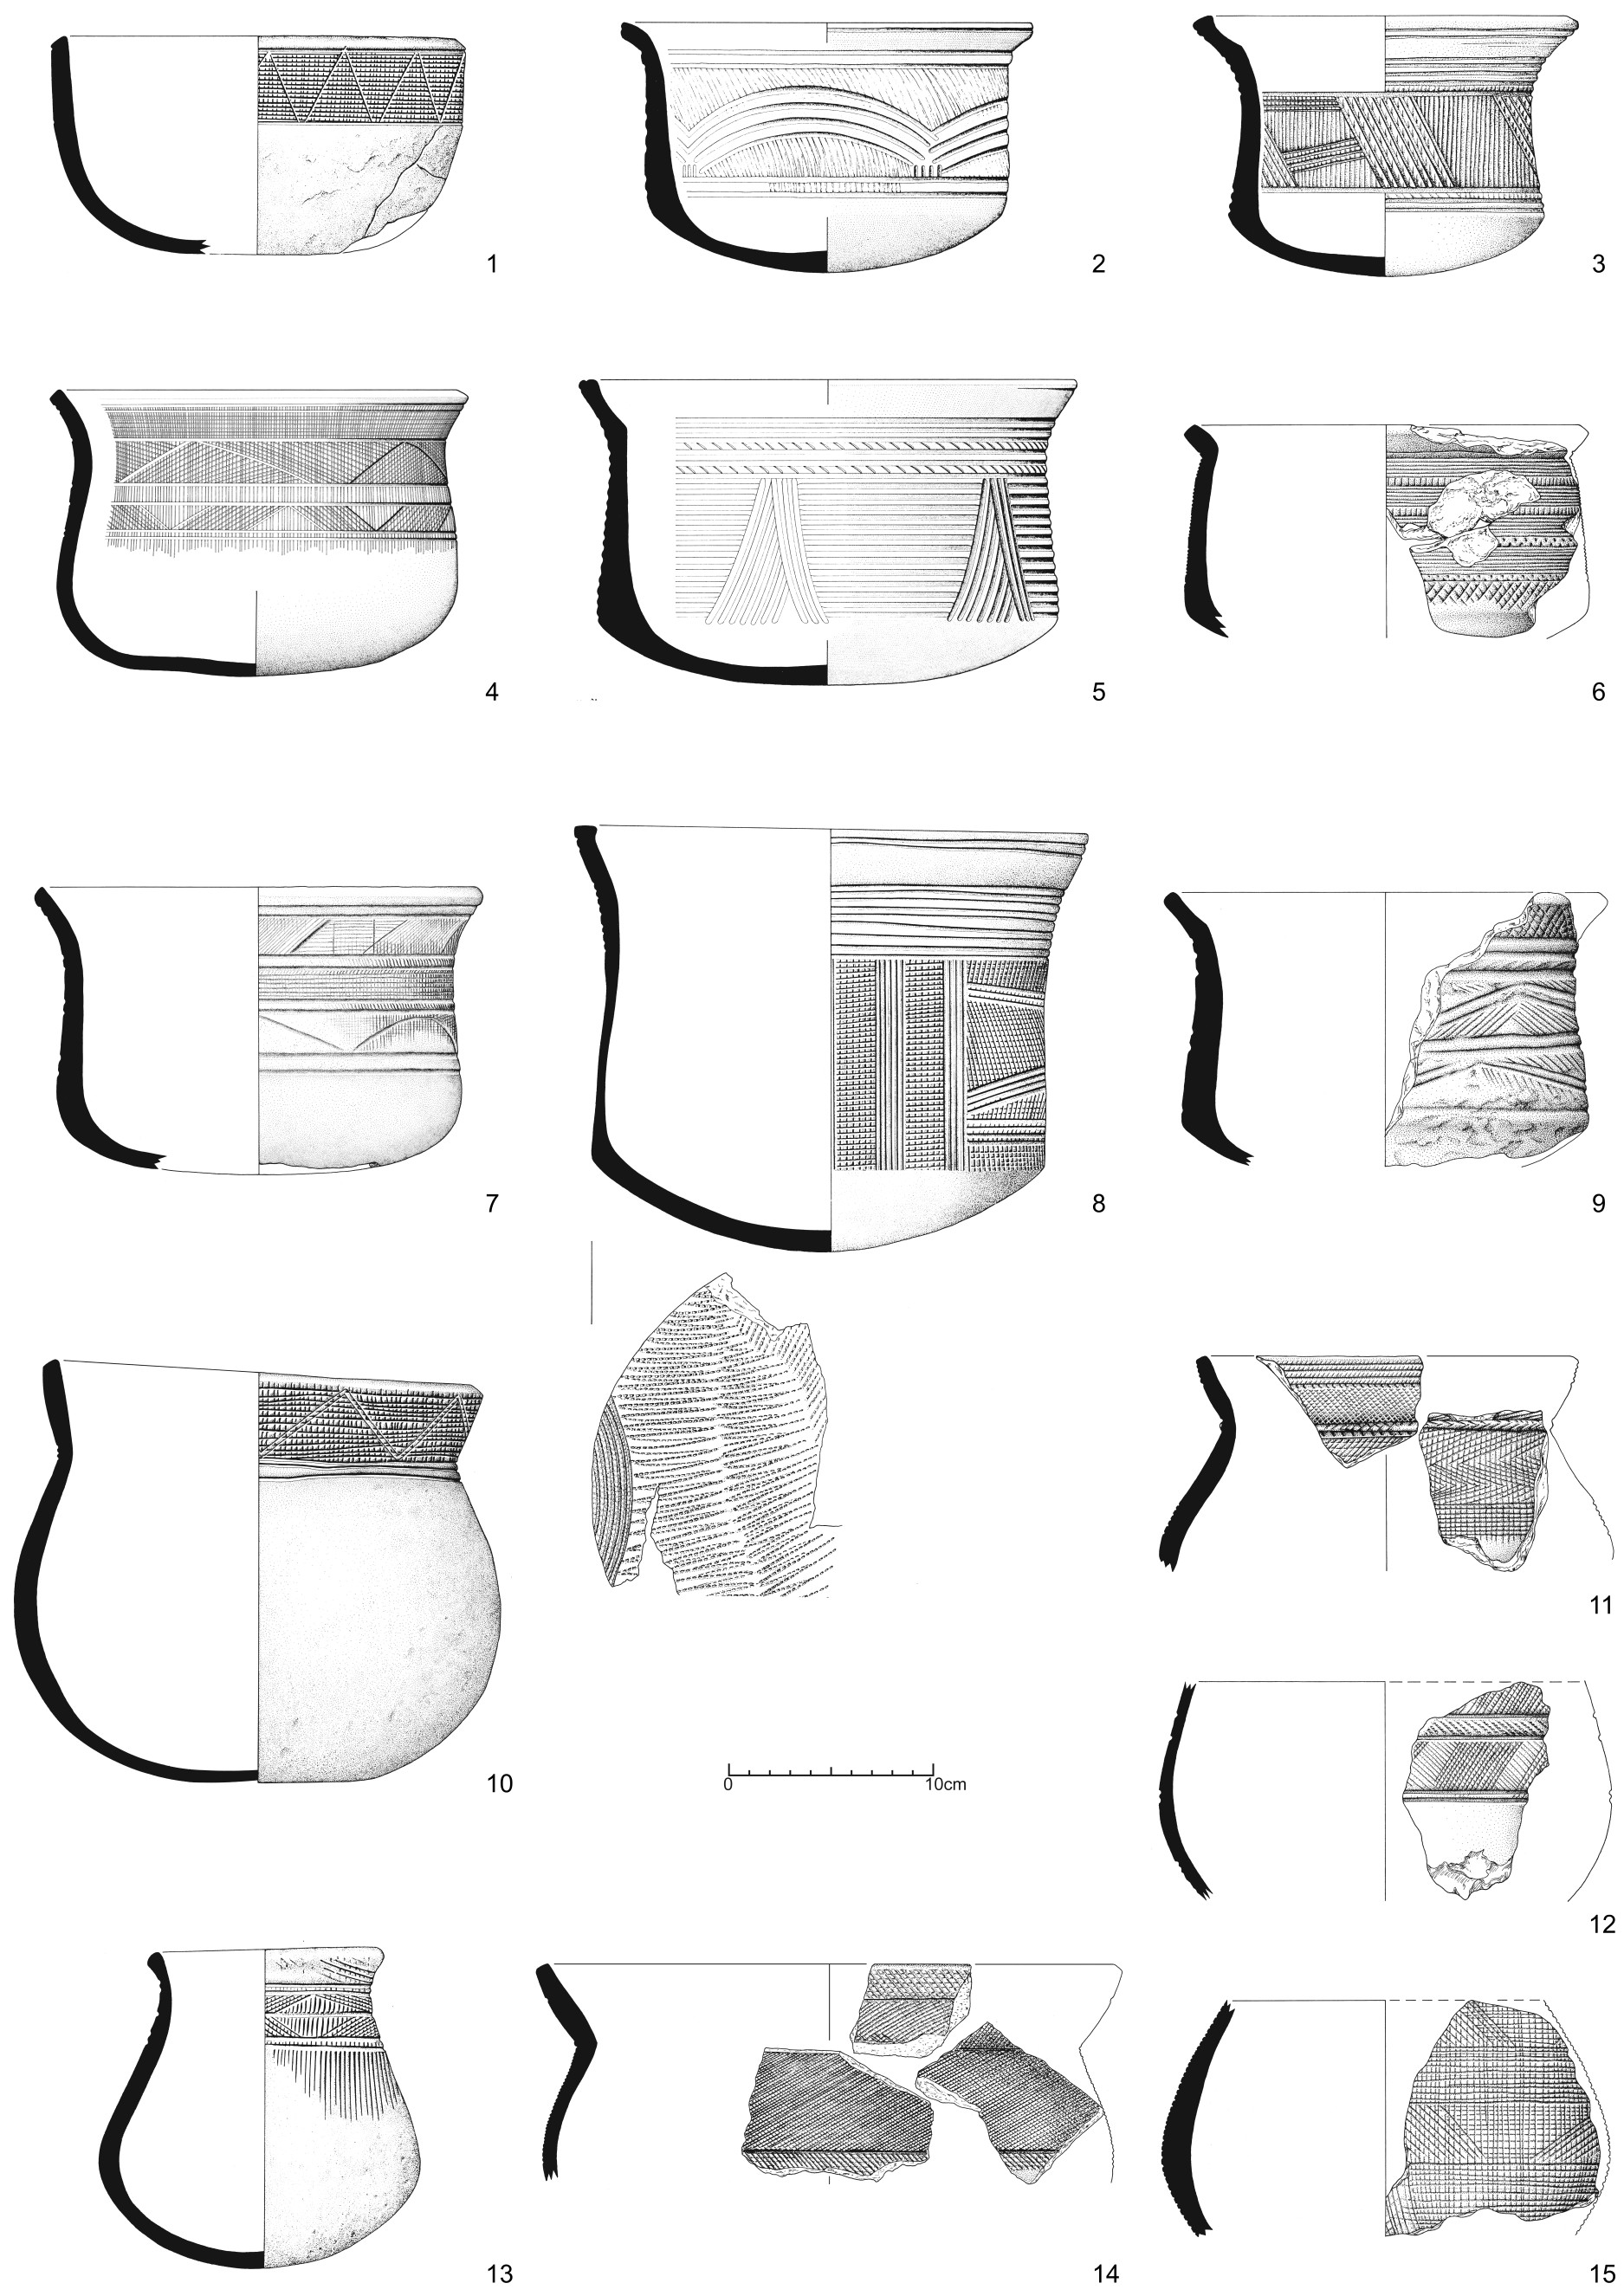
\includegraphics[width=\textwidth]{fig/PKM-Typen.pdf}
	\caption{Pikunda-Munda-Gruppe: Typvertreter.\\1:~Taf.~92.5; 2:~Taf.~91.1; 3:~Taf.~50.1; 4:~Taf.~92.7; 5:~Taf.~91.5; 6:~Taf.~32.1; 7:~Taf.~91.7; 8:~Taf.~44.3; 9:~Taf.~94.1; 10:~Taf.~93.3; 11:~Taf.~51.1; 12:~Taf.~46.20; 13:~Taf.~92.8; 14:~Taf.~45.1; 15:~Taf.~51.3.}
	\label{fig:PIKMUN_TypVertreter}
\end{figure*}

\paragraph{Formen}\hspace{-.5em}|\hspace{.5em}%
Das bestimmende Charakteristikum der Pikunda-Munda-Gruppe sind hohe Schalen mit Bauch"-umbruch oder -knick, ausbiegendem Rand und rundem Boden vom Typ E3 sowie F3 (Abb. \ref{fig:PIKMUN_TypVertreter}.2--9). Daneben sind nur wenige weitere Gefäßformen bekannt (Abb.~\ref{fig:PIKMUN_TypVertreter}.1,10--15). Die beiden charakteristischen Schalenformen machen jeweils 40--43\,\% aller sicher zu bestimmenden Gefäßformen der Pikunda-Munda-Gruppe aus. Gefäße mit geschweifter Wandung, die keinen dezidiert ausgearbeiteten Halsbereich aufweisen, ließen sich bei 10\,\% aller GE der Pikunda-Munda-Gruppe nachweisen (Typ~E1; Abb.~\ref{fig:PIKMUN_TypVertreter}.10--12,14--15).\vspace{1em}

\begin{figure*}[tb]
	\noindent\begin{minipage}[b]{\columnwidth}
		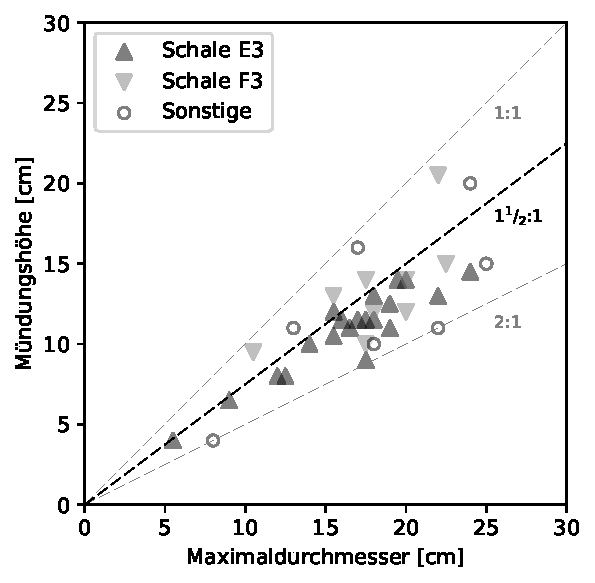
\includegraphics[width=\columnwidth]{fig/PKM_Proportionen.pdf}
		\captionof{figure}{Pikunda-Munda-Gruppe: Proportionen der Gefäße.\label{fig:PIKMUN_Proportionen}}\vspace{1em}
		\captionof{figure}{Pikunda-Munda-Gruppe: Kalibierung der \textsuperscript{14}C-Datierungen für die Gruppen I und II (Siehe Anlage~2).\label{fig:PIKMUN_14C}}\vspace{1em}
	\end{minipage}\hfill
	\noindent\begin{minipage}[b]{\columnwidth}
	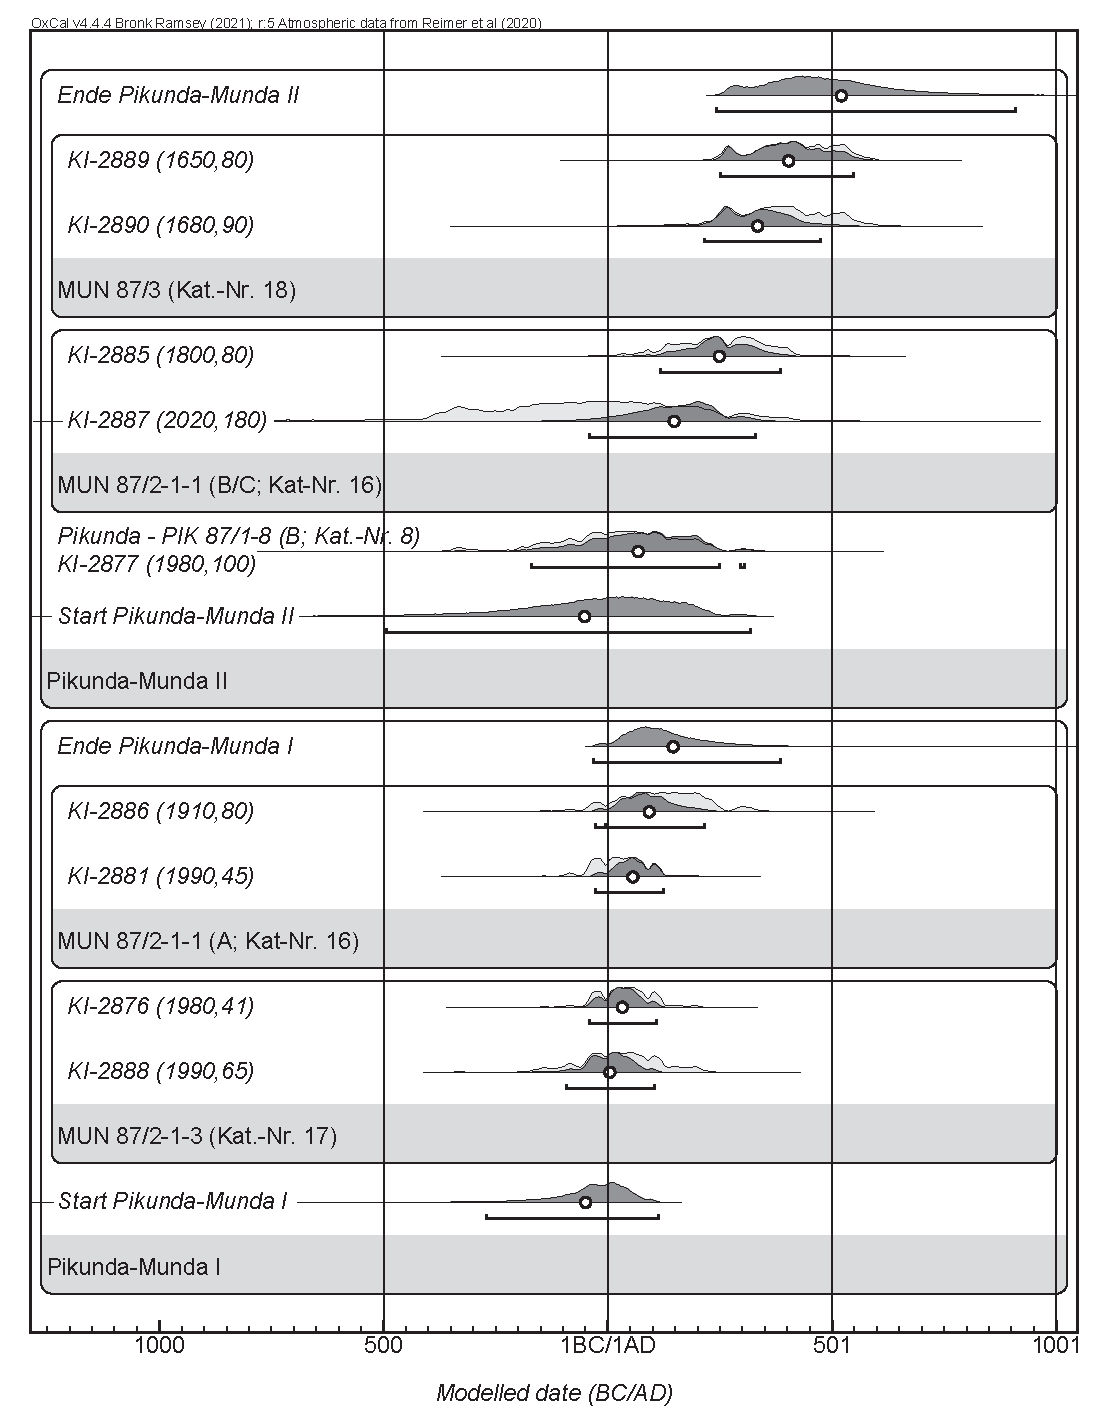
\includegraphics[width=\columnwidth]{fig/PKM_14C.pdf}
	\end{minipage}
\end{figure*}

Schalenförmige Gefäße mit konvexer Wandung (Typ~I; Abb.~\ref{fig:PIKMUN_TypVertreter}.1) sowie hohe Gefäße mit ausgeprägtem Halsbereich (Typ~B; Abb.~\ref{fig:PIKMUN_TypVertreter}.13) ließen sich lediglich als Einzelfunde beobachten. Die Schalen sind im Schnitt etwa anderthalb mal so breit wie hoch, wobei die Schalen des Typs E3 tendenziell etwas flacher als jene des Typs F3 sind (Abb.~\ref{fig:PIKMUN_Proportionen}). Der Mündungsdurchmesser der Schalen vom Typ E3 liegt zwischen 6 und 31\,cm, während er bei den Schalen vom Typ F3 zwischen 11 und 31\,cm schwankt. Die Höhe der Schalen variiert zwischen 4 und 14,5\,cm (Typ~E3) beziehungsweise 9,5 und 20,5\,cm (Typ~F3). Während die Ränder deutlich über den minimalen Gefäßdurchmesser hinausragen, im Schnitt um knapp 16\,\%, ist der maximale Durchmesser im Bereich der Gefäßwandung, der direkt zum Gefäßboden umleitet, nur etwa 5--10\,\% größer als der Minimaldurchmesser.

Mit Bezug auf die Ausgestaltung der Randlippen ließen sich im Material der Pikunda-Munda-Gruppe zu in etwa gleichen Anteilen runde (M1; 32\,\%; Abb. \ref{fig:PIKMUN_TypVertreter}.13), gerade (M3; 32\,\%; Abb. \ref{fig:PIKMUN_TypVertreter}.5,8) sowie schräg nach außen (M5; 27\,\%; Abb.~\ref{fig:PIKMUN_TypVertreter}.1,3--4,6--7,9--11) abgestrichene Mündungsabschlüsse beobachten. Gerillte Randlippen (M4) fanden sich nur bei 3\,\% der Stücke (Abb.~\ref{fig:PIKMUN_TypVertreter}.2). Die Ränder selbst sind regelhaft ausbiegend. Zu etwa gleichen Anteilen lassen sich gerade (B1; 29\,\%; Abb.~\ref{fig:PIKMUN_TypVertreter}.6,8--11) sowie konkav (B2; 30\,\%; Abb.~\ref{fig:PIKMUN_TypVertreter}.2,4,7,13) und konvex (B3; 26\,\%; Abb.~\ref{fig:PIKMUN_TypVertreter}.3,5) ausbiegende Ränder beobachten. Nur selten sind gerade aufsteigende Ränder zu beobachten (A1; 9\,\%, Abb.~\ref{fig:PIKMUN_TypVertreter}.1). Die Böden sind mit wenigen Ausnahmen, die allesamt eher als unbeabsichtigte Einzelfälle denn als beabsichtigte Produkte des Töpfereiprozesses angesehen werden können, rund ausgeführt (Abb.~\ref{fig:PIKMUN_TypVertreter}.1, 10). Der Bodentyp B1 findet sich bei 86\,\% der 64~GE, bei denen die Form des Bodens aufgenommen werden konnte.

\paragraph{Verzierungen}\hspace{-.5em}|\hspace{.5em}%
Pikunda-Munda-Keramik zeichnet sich durch eine im Grundsatz sehr klare und homogene Verzierungspraxis aus. Während die Gefäßunterteile und runden Böden nur sehr selten verziert sind, in einigen Fällen lässt sich Kamm-Wiegeband beobachten (Tab.~\ref{tab:Verzierungselemente}: 04.2; 2\,\%; Abb.~\ref{fig:PIKMUN_TypVertreter}.8), weisen die Oberteile eine vornehmlich durch horizontale Bänder gegliederte, umfangreiche Verzierung auf (Anlage~4\subref{fig:PIKMUN_Verz}). Zusammengenommen machen Rillen (Tab.~\ref{tab:Verzierungselemente}: 01) und Riefen (Tab.~\ref{tab:Verzierungselemente}: 02) 82\,\% aller an GE der Pikunda-Munda-Gruppe beobachteten Verzierungselementen aus. Horizontale Rillen (Tab.~\ref{tab:Verzierungselemente}: 02.1) finden sich vornehmlich außen auf dem Rand sowie Bauch der Gefäße machen 34\,\% aller Verzierungen aus, gefolgt von dem aus sich überkreuzenden Rillen aufgebauten Schachbrettmuster (24\,\%; Tab.~\ref{tab:Verzierungselemente}: 01.1--4). Neben diesen regelhaft zu beobachtenden Verzierungselementen fällt die Nutzung von horizontalen Reihen aus kleinen, häufig diagonal gesetzten Eindrücken auf (Tab.~\ref{tab:Verzierungselemente}: 04.12; 6\,\%). Grundsätzlich sind fast alle im Katalog der Verzierungselemente aufgenommen Variationen von Rillen (Tab.~\ref{tab:Verzierungselemente}: 01) und Riefen (Tab.~\ref{tab:Verzierungselemente}: 02) auf den GE der Pikunda-Munda-Gruppe vertreten. Durch die Verzierung der GE wird insbesondere der Rand sowie der Gefäßbauch betont. Auffällig ist dabei eine Tendenz zu horizontalen Bändern und flächigen Mustern sowie eine durch vertikal gesetzte Verzierungselemente erzeugte, metopenartige Strukturierung der Verzierung. 

\begin{table*}[tb!]
	\centering{\footnotesize \begin{sftabular}{@{}lccc|ccccccc@{}}
			\toprule
			\multirow{2}{*}{} & \multicolumn{2}{c}{\textbf{PKM}} & \multirow{2}{*}{\textbf{LKW 186}} & \multirow{2}{*}{\textbf{IMB}} & \multirow{2}{*}{\textbf{BON}} & \multirow{2}{*}{\textbf{ING}} & \multirow{2}{*}{\textbf{LOK}} & \multirow{2}{*}{\textbf{BKE}} & \multirow{2}{*}{\textbf{LUS}} & \multirow{2}{*}{\textbf{LNG}} \\
			& \multicolumn{1}{c}{\textbf{I}} & \multicolumn{1}{c}{\textbf{II}} &  & & & & & &  \\
			\midrule
			Topf mit Schulterabsatz (Typ~C) &  &  & $\circ$ & $\bullet$ & $\bullet$ & $\circ$ &  &  &  &  \\
			Schale mit Bauchknick (Typ E3 \& F3) & $\circ$ & $\bullet$ & & &  &  &  & $\circ$ &  &  \\
			Rundbodig (B1--3) & $\bullet$ & $\bullet$ &  &  &  &  &  & $\bullet$ & &  \\
			Flachbodig (B1--14) & $\circ$ &  & $\bullet$  & $\bullet$  & $\bullet$ & $\bullet$ & $\bullet$ & $\bullet$ & $\bullet$ & $\bullet$ \\
			Kamm-Wiegeband (Tab.~\ref{tab:Verzierungselemente}: 04.1) &  & $\bullet$ &  & $\bullet$ & $\bullet$ & $\bullet$ &  & & & \\
			\textit{Schachbrett}-Muster (Tab.~\ref{tab:Verzierungselemente}: 01.1--4) &  & $\bullet$ &  &  &  &  & $\bullet$ & &  & $\bullet$ \\
			\textit{Fabric} 1--2 & $\bullet$ & $\bullet$ & $\circ$ & $\circ$  & $\circ$  & $\circ$  & $\bullet$ & $\circ$ & $\circ$ & $\circ$ \\
			\bottomrule
	\end{sftabular}}
	\caption{Pikunda-Munda-Gruppe: Gegenüberstellung von formalen Merkmalen und Verzierungspraxis der postulierten Untergruppen der Pikunda-Munda-Gruppe zum Inventar aus LKW~87/186 (Kat.-Nr.~19) sowie zeitgleichen Stilgruppen und der älteren Imbonga-Gruppe des Inneren Kongobeckens.\\$\bullet$ vorhanden, $\circ$ fraglich. \\ PKM: Pikunda-Munda, LKW 186: Inventar des Komplexes LKW~87/186 (Kat.-Nr.~19), IMB: Imbonga (\textsc{Wotzka} 1995: 59--68), BON: Bonkake (ebd. 68--73),\\ING: Ingende (ebd. 73--78), LOK: Lokondola (ebd. 84--89), BKL: Bokele (ebd. 100--104), LUS: Lusako (ebd. 104--107), LNG: Lingonda (ebd. 108--115).}
	\label{tab:PIKMUN_Vgl}
\end{table*}

\paragraph{Datierung}\hspace{-.5em}|\hspace{.5em}%
Mit Keramik des Pikunda-Munda-Stils sind neun Radiokohlenstoffdatierungen assoziiert (Tab.~\ref{tab:14Cdatings}). Diese stammen ausnahmslos aus den für die Beschreibung der Stilgruppe zentralen Ausgrabungen in Pikunda am \mbox{Sangha} (Fpl.~255) und Munda am \mbox{Likwala}-\mbox{aux}-\mbox{Herbes} (Fpl.~304). Die Grabung MUN~87/2-1-1 (Kat-Nr.~16) in Munda (Fpl.~304) erbrachte einen stratifizierten Befund, der eine Differenzierung des keramischen Materials der Pikunda-Munda-Gruppe in zwei Unterstile andeutet. Zwei, klar durch eine verziegelte Lehmwanne voneinander getrennte Grubenverfüllungen erbrachten jeweils homogene Inventare. Beide fallen grundsätzlich in das Spektrum der Pikunda-Munda-Gruppe, da die charakteristischen Schalenformen das bestimmende Merkmal sind, weisen jedoch auch Abweichungen zueinander auf. In der stratigrafisch älteren Verfüllung A (siehe Kat-Nr.~16) fanden sich ausnahmslos Pikunda-Munda-Schalen mit einem runden, geschweiften Umbruch des Gefäßbauches (Typ~E3; Taf.~91.6--8). Diese entsprechenden Schalen der Untergruppe I der Pikunda-Munda-Gruppe zeichnen sich durch eine Verzierung aus, die fast ausschließlich aus flachen Rillen bestehenden horizontalen Bändern (Tab.~\ref{tab:Verzierungselemente}: 02.1) sowie Schachbrettmustern (Tab.~\ref{tab:Verzierungselemente}: 01.1) auf den Rändern und Bauchbereichen der Gefäße besteht. Ein diesem morphologisch wie ornamental entsprechendes Inventar fand sich in der nur 0,35\,m nördlich anschließenden Grube MUN~87/2-1-3 (Kat.-Nr.~17). Im Unterschied zu den Gefäßen des unteren Verfüllungsbereiches A in MUN~87/2-1-1 erbrachte der obere Verfüllungsbereich C ein Inventar, welches größtenteils aus Schalen mit einem deutlich ausgeprägten Bauchknick besteht (Typ~F3; Taf.~91.1--5). Dieses ist repräsentativ für die Untergruppe II des Pikunda-Munda-Stils. Die Schalen weisen eine leicht andere Ornamentik auf, die auf tieferen Rillen und flächigem Wiegeband mit Klinge oder Kamm basiert (Tab.~\ref{tab:Verzierungselemente}: 04.1--2). Die durch die Grabung PIK~87/1 (Kat.-Nr.~8) in Pikunda am \mbox{Sangha} (Fpl.~255) erschlossene Grube B1/B2 erbrachte ebenfalls ausschließlich Pikunda-Munda-Schalen mit einem Profilknick vom Typ F3. Die aus diesen Beobachtungen ableitbaren Untergruppen der Pikunda-Munda-Gruppe weisen trennende wie verbindende Merkmale auf (Tab.~\ref{tab:PIKMUN_Vgl}). Die Schalenformen vom Typ E3 mit ihrem auffällig abgerundeten Bauchumbruch (Abb.~\ref{fig:PIKMUN_TypVertreter}.4,7) stehen dabei den Schalen vom Typ F3 gegenüber, die einen deutlichen und teilweise scharfen Bauchknick aufweisen (Abb.~\ref{fig:PIKMUN_TypVertreter}.3--4,5--6,8--9).

\begin{figure*}[p]
	\centering
	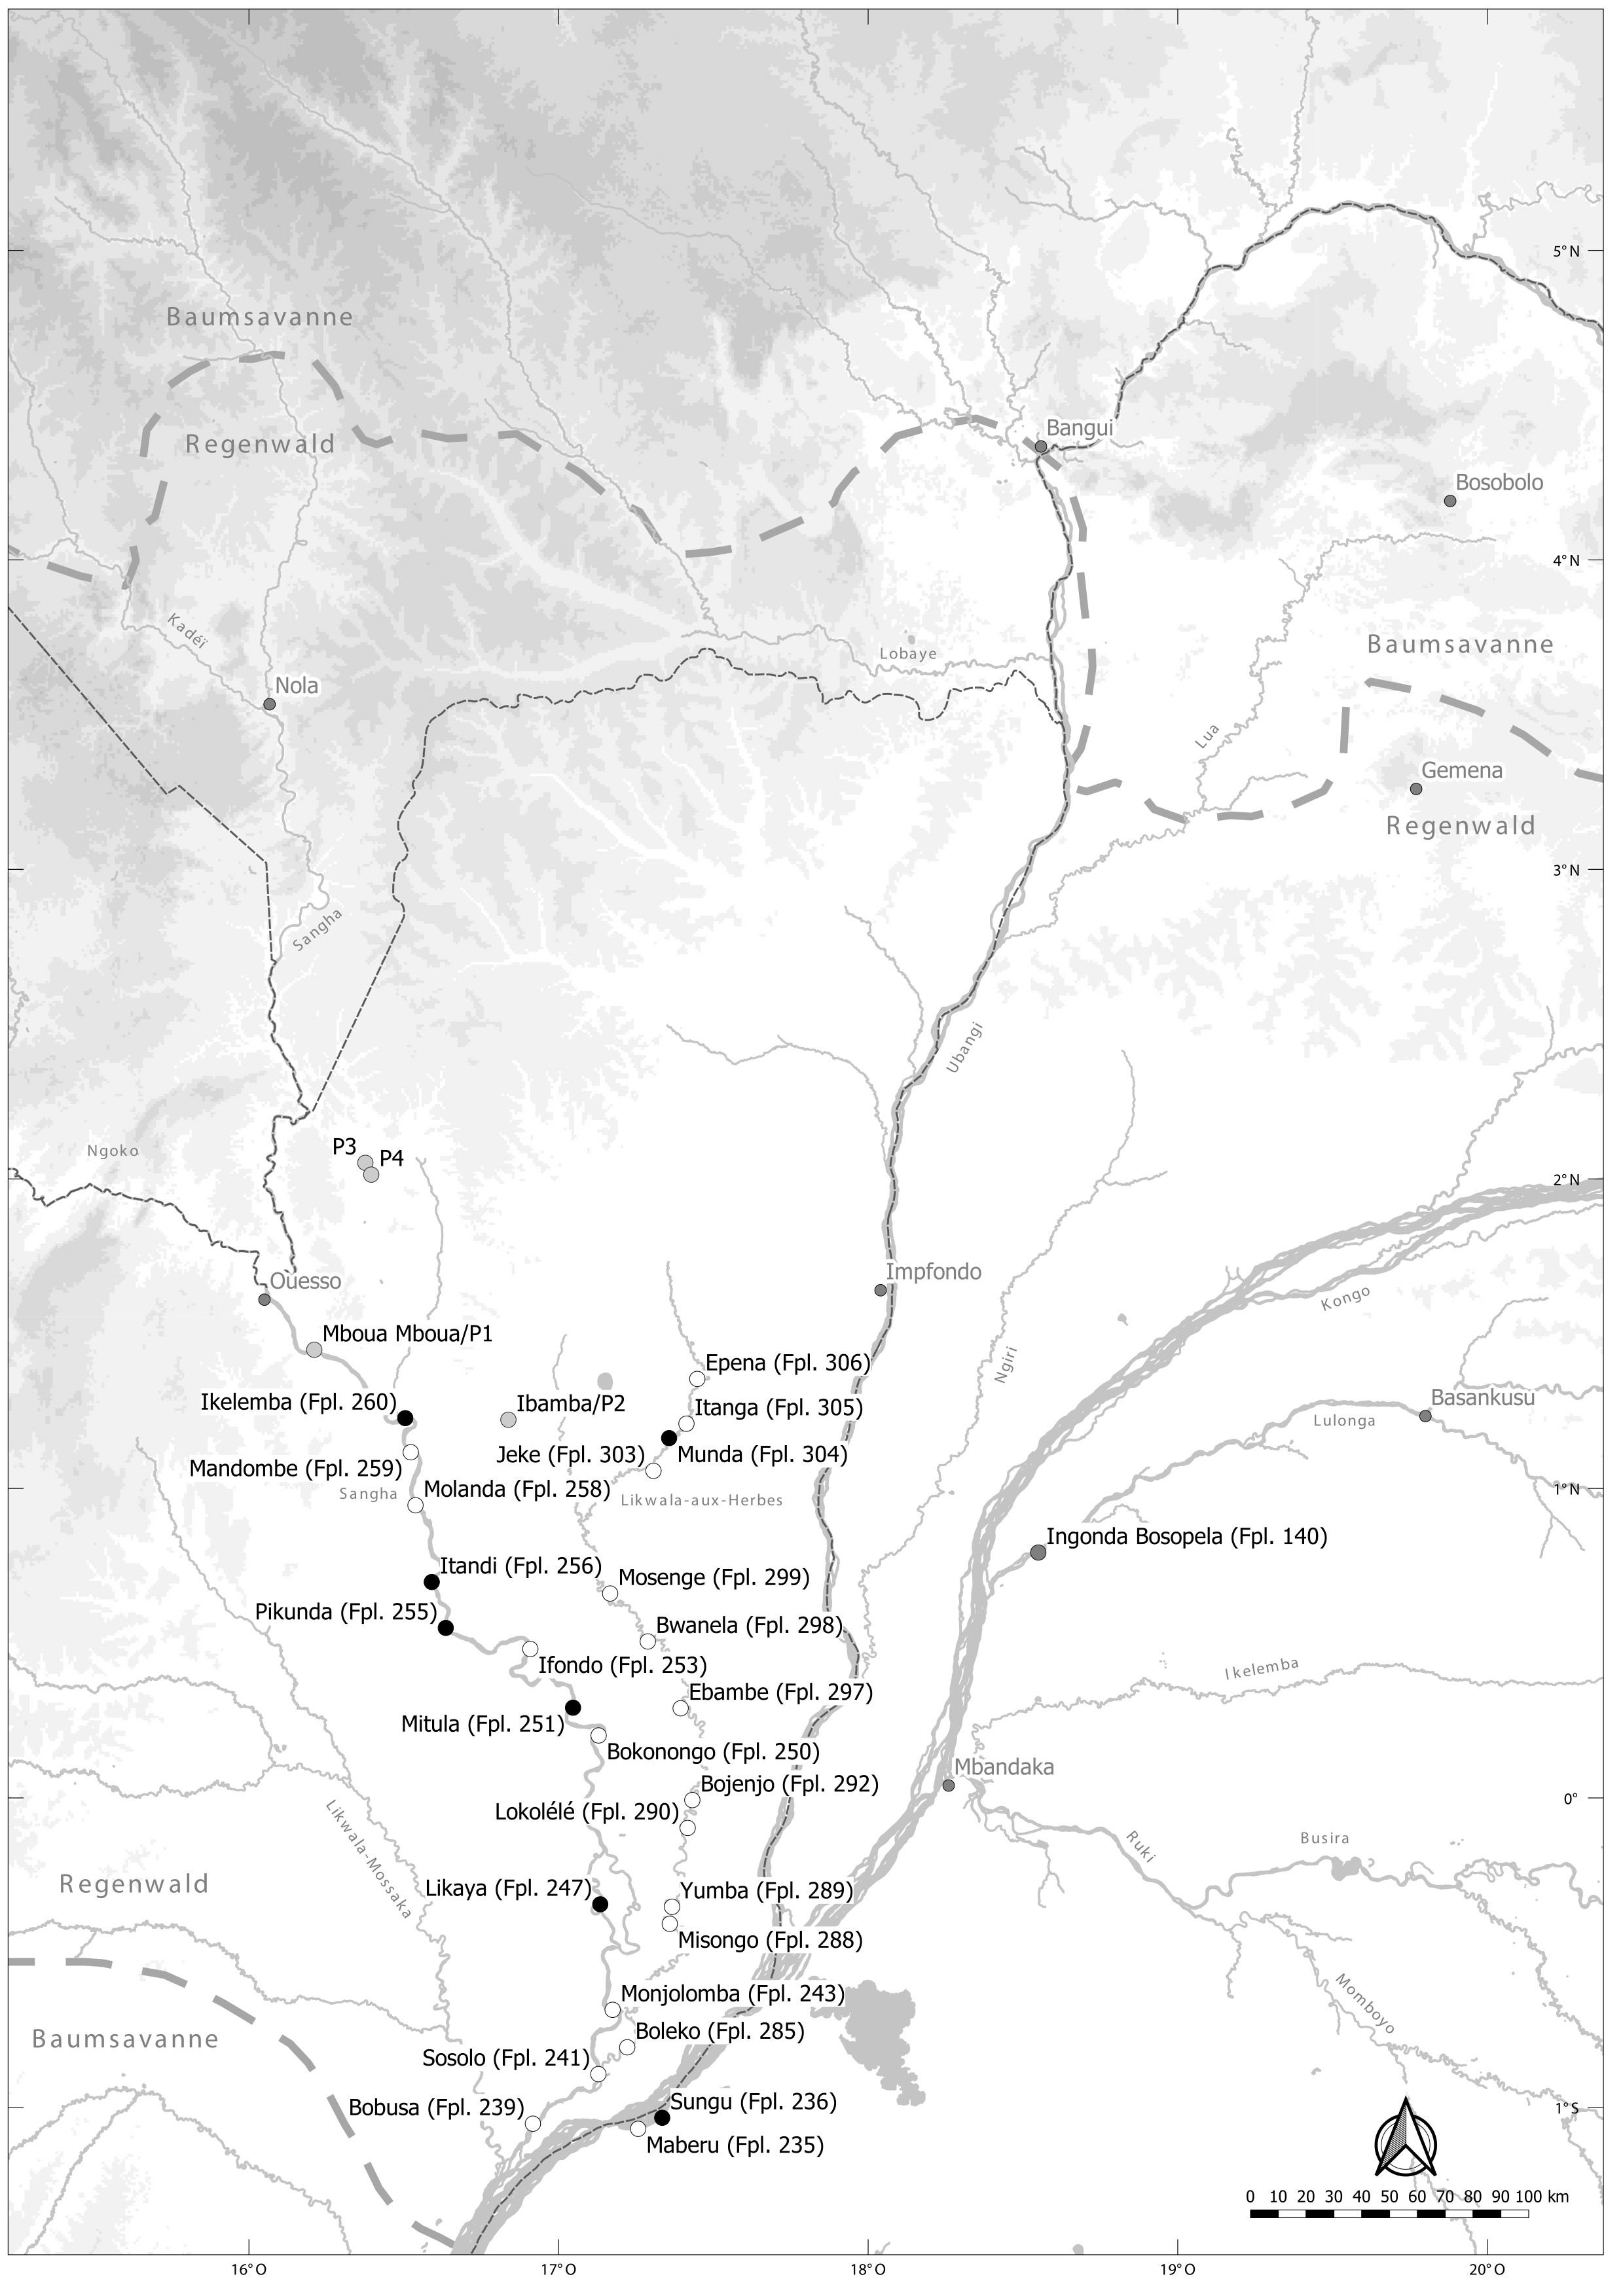
\includegraphics[width=\textwidth]{fig/PKM_Verbreitung.pdf}
	\caption{Pikunda-Munda-Gruppe: Verbreitung \parencites[grau nach][119 Anm.~4, 531 Taf.~97.5]{Wotzka.1995}[114 Abb.~42]{Gillet.2013}.}
	\label{fig:PIKMUN_Verbreitung}
\end{figure*}

Der Beginn des Pikunda-Munda-Stils kann auf Basis der vorliegenden Datierungen in das 2.--1.~Jh. v.~Chr. datiert werden (Abb.~\ref{fig:PIKMUN_14C}), wenn die Datierung KI-2887 (Tab.~\ref{tab:MUN87-211_14C-Daten}; Anlage 2) ausgelassen wird, das diese einen besonders hohen Standardfehler aufweist. Die jüngsten Radiokohlenstoffdatierungen für Pikunda-Munda-Keramik stammen aus dem Befund MUN~87/3 in Munda am \mbox{Likwala}-\mbox{aux}-\mbox{Herbes} und fallen in das 2.-6.~Jh. n.~Chr. (Abb.~\ref{fig:PIKMUN_14C}: KI-2889, KI-2890).\footnote{Die Keramik dieses Befundes spiegelt mit einer Schale vom Typ F3 (Abb.~\ref{fig:PIKMUN_TypVertreter}.9) die formalen Charakteristika der Untergruppe II wider.} Bereits \textsc{Wotzka} (1995: 107 Anm.~4) hat auf den Umstand hingewiesen, dass sich gewisse Merkmale der Pikunda-Munda-Keramik auch bei keramischen Stilgruppen des Inneren Kongobeckens beobachten lassen (Tab.~\ref{tab:PIKMUN_Vgl}).\footnote{Der Pikunda-Munda-Gruppe auf Merkmalsebene nahestehende Gefäße fanden sich im Zusammenhang mit Feldarbeit an der Fundstelle Yatou in Kamerun an der Mündung des Sanaga-Flusses (siehe Kap.~\ref{sec:Kamerun}). Die beiden aus dem Befund YAT~99/1 vorliegenden Radiokohlenstoffdatierungen decken das 1.~Jh. v.~Chr. bis 1.~Jh. n.~Chr. (KIA-12942) sowie das 7.--9.~Jh. n.~Chr. (KIA-12941) ab. Gerade die ältere der beiden Datierungen lässt sich leicht mit dem hier postulierten Alter für die Pikunda-Munda-Gruppe in Einklang bringen. Eine detaillierte Auswertung der Befunde und Funde aus Yatou steht gegenwärtig aus (Kap.~\ref{sec:Kamerun}).} Während die für den Pikunda-Munda-Stil charakteristischen Schalen keine Entsprechung im Fundgut des Inneren Kongobeckens finden, so ist Kamm-Wiegeband-Dekor ein starkes Merkmal der ältesten Stile Imbonga, Bonkake und Ingende (ebd. 59--78). Auch ein aus überkreuzenden, feinen Ritzlinien bestehendes Dekor findet sich in zeitgleichen Stilen, allen voran der Lokondola-Gruppe.\footnote{Eine Scherbe dieses Stils fand sich auch in der älteren, in Pikunda erfassten Grube (Kat.-Nr.~8).} Zusammenfassend lässt sich festhalten, dass der Pikunda-Munda-Stil stilistisch einige lose Anbindungen an die zeitgleichen Stilgruppen des Inneren Kongobeckens aufweist, jedoch mit Blick auf die Keramiktechnologie nicht von der weiter östlich gefunden Keramik unterscheidbar ist. Zusammenfassend kann die Pikunda-Munda-Keramik gegenwärtig mit hinreichender Sicherheit in das 2.--1.~Jh. v.~Chr. bis 5.--6.~Jh. n.~Chr. datiert werden.

\paragraph{Verbreitung}\hspace{-.5em}|\hspace{.5em}%
Die Verbreitung der Pikunda-Munda-Keramik (Abb.~\ref{fig:PIKMUN_Verbreitung}) beschränkt sich auf die Flussläufe des \mbox{Sangha} und \mbox{Likwala}-\mbox{aux}-\mbox{Herbes} von deren Mündung in den Kongo bis Ikelemba am \mbox{Sangha} (Fpl.~260) beziehungsweise Epena am \mbox{Likwala}-\mbox{aux}-\mbox{Herbes} (Fpl.~306).\footnote{Erst im Zuge der Feldarbeiten der Arbeitsgruppe um Richard Oslisly wurde die Fundstelle Pikunda (Fpl.~255) in den frühen 2010er Jahren wieder aufgesucht \parencite[211 Abb.~1, 212\,f. Tab.~1 Nr.~25--26]{MorinRivat.2014}.} Material des Pikunda-Munda-Stils fand sich auch in Maberu (Fpl.~235) und Sungu (Fpl.~236) am Kongo, etwa 50\,km nordöstlich der Mündung des \mbox{Sangha}. Das Verbreitungsgebiet reicht folglich etwa 250\,km in Nord--Süd- und etwa 110\,km in Ost--West-Richtung.

Innerhalb der Komplexe aus Oberflächenabsammlungen war eine sichere Ansprache von Scherben des Pikunda-Munda-Stils aufgrund starker Fragmentierung und hoher Erosion der Oberflächen selten möglich. Zudem erschwerte die teils recht einfache Rillen- und Riefenverzierung (Tab.~\ref{tab:Verzierungselemente}: 01--02) die sichere Ansprache kleinerer Stücke. Daraus resultiert, dass große Teile der aus Oberflächenkomplexen stammenden Stücke lediglich unter Vorbehalt dem Pikunda-Munda-Stil zugeordnet werden konnten. Diese Unsicherheiten spiegeln sich auch im Verbreitungsgebiet der Pikunda-Munda-Gruppe wider (Abb.~\ref{fig:PIKMUN_Verbreitung}). Entlang des \mbox{Likwala}-\mbox{aux}-\mbox{Herbes} sowie im \mbox{Sangha}-Mündungsgebiet lagen häufig keine ausreichenden Merkmale für eine sichere Ansprache vor, und manche Scherben konnten nur unter Vorbehalt angesprochen werden.

Aus dem von \textsc{Wotzka} (1995: 119 Anm. 4, 531 Taf.~97.5) bearbeiteten Inneren Kongobecken liegt ein, im Zuge von Surveys gefundenes Gefäß aus Ingonda Bosopela am unteren Lulonga (Fpl. 140) vor.\footnote{Dabei handelt es sich um das Fragment einer Schale mit ausbiegendem Rand, gerader oberer Wandung und einem auffälligen, runden Bauchumbruch, das dem Gefäßtyp E3 zugeordnet werden kann. Die Verzierung dieses Stücks besteht aus Riefen, die ein aus feinen, vertikalen Rillen bestehendes Band einrahmen, das zudem von girlandenartigen Rillen überlagert wird (Tab.~\ref{tab:Verzierungselemente}: 02.1, 02.2, 02.5). Der Randabschluss weist feine, diagonal sitzende Rillen oder Eindrücke auf \parencite[Tab.~\ref{tab:Verzierungselemente}: 02.3 oder 04.12; 119 Anm. 4, 531 Taf.~97.5]{Wotzka.1995}.} Des Weiteren sind potenzielle Scherben der Pikunda-Munda-Gruppe an vier Plätzen belegt, die im Rahmen ökologischer Untersuchungen im Norden der Republik Kongo erschlossen wurden \parencite[114 Abb.~42; Abb.~\ref{fig:PIKMUN_Verbreitung}]{Gillet.2013}. Die Fundstellen zeichnen sich neben den keramischen Funden durch bei Bohrungen erfasste Holzkohlekonzentrationen aus (ebd. 94 Tab.~14). Da die Ansprache lediglich anhand der veröffentlichten Fotografien erfolgte, kann eine Zuweisung nur unter starken Vorbehalten postuliert werden. Akzeptierte man diese Fundpunkte jedoch, so würde sich das Verbreitungsgebiet der Pikunda-Munda-Gruppe um etwa 50\,km nach Norden ausweiten, auf eine Ausdehnung von etwa 300\,km in Nord--Süd-Richtung.